% !TeX encoding = UTF-8 Unicode
\documentclass[a4paper,12pt]{article}
\usepackage[english]{babel}
\usepackage[english]{isodate}
\usepackage{graphicx}
\usepackage{hyperref}
\usepackage{centernot}
\usepackage{xfrac}
\usepackage{mathtools}
\usepackage{enumitem}
\usepackage{fancyhdr}
\usepackage{lastpage}
\usepackage{xcolor}
\usepackage{changepage}
\usepackage{amsthm}
\usepackage{amsfonts}
\usepackage{amsmath}
\usepackage{amssymb}
\usepackage{soul}
\usepackage{float}
\usepackage{centernot}
\usepackage{tcolorbox}
\usepackage{titling}
\usepackage{caption}
\usepackage{subcaption}
\usepackage{etoolbox}
\usepackage{listings}
\usepackage{biblatex}
\usepackage{csquotes}
\usepackage{titlesec}
\usepackage{tikz}
\usetikzlibrary{trees}

\addbibresource{bibliography.bib}

\patchcmd{\section}{\bfseries}{\bfseries\boldmath }{}{}
\patchcmd{\subsection}{\bfseries}{\bfseries\boldmath }{}{}
\patchcmd{\subsubsection}{\bfseries}{\bfseries\boldmath }{}{}

\hypersetup{
  colorlinks=True,
  urlcolor=blue,
  citecolor=red,
  menucolor=black,
}

\renewcommand{\UrlFont}{\ttfamily\footnotesize}

\lstdefinelanguage{futhark}
{
  % list of keywords
  morekeywords={
  do,
  else,
  for,
  if,
  in,
  include,
  let,
  loop,
  then,
  type,
  val,
  while,
  with,
  module,
  def,
  entry,
  local,
  open,
  import,
  assert,
  match,
  case,
  },
  sensitive=true, % Keywords are case sensitive.
  morecomment=[l]{--}, % l is for line comment.
  morestring=[b]" % Strings are enclosed in double quotes.
}


\lstset{
  language=futhark,
  showspaces=false,
  showstringspaces=false,
  mathescape=true,
  aboveskip=0pt,
  belowskip=6pt,
  numberstyle=\tiny,
  numbers=left, 
  firstnumber=1,
  numberfirstline=true,
  tabsize=4,
  breaklines=true,
}

\newcommand\LAST{\text{LAST}}
\newcommand\defiff{\mathrel{\stackrel{\makebox[0pt]{\mbox{\normalfont\tiny def}}}{\iff}}}
\newcommand\defeq{\mathrel{\stackrel{\makebox[0pt]{\mbox{\normalfont\tiny def}}}{=}}}
\newcommand\concat{\: \mathrlap{+} \: +}
\newcommand\map{\textbf{map}\ }
\newcommand\reduce{\textbf{reduce}\ }
\theoremstyle{definition}
\newtheorem{definition}{Definition}[section]
\newtheorem{proposition}{Proposition}[section]
\newtheorem{corollary}{Corollary}[section]
\newtheorem*{remark}{Remark}
\newtheorem{lemma}{Lemma}[section]
\newtheorem{theorem}{Theorem}
\newtheorem{algorithm}{Algorithm}[section]
\newtheorem{example}{Example}[section]
\newtheorem{conjecture}{Conjecture}[section]
\DeclareMathOperator{\sign}{sign}
\newcommand\doubleplus{+\kern-1.3ex+\kern0.8ex}
\newcommand\mdoubleplus{\ensuremath{\mathbin{+\mkern-10mu+}}}

\newcommand{\id}[1]{\ensuremath{\mathit{#1}}}
\newcommand{\kw}[1]{\ensuremath{\mathtt{#1}}}
\newcommand{\Let}{\kw{let}}
\newcommand{\In}{\kw{in}}
\newcommand{\If}{\kw{if}}
\newcommand{\Then}{\kw{then}}
\newcommand{\Else}{\kw{else}}
\newcommand{\Filter}{\kw{filter}}
\newcommand{\Or}{\kw{or}}
\newcommand{\Groupby}{\kw{groupby}}
\newcommand{\Partition}{\kw{partition}}
\newcommand{\Scatter}{\kw{scatter}}
\newcommand{\Hist}{\kw{hist}}
\newcommand{\Map}{\kw{map}}
\newcommand{\Sum}{\kw{sum}}
\newcommand{\Mod}{\kw{mod}}
\newcommand{\Fst}{\kw{fst}}
\newcommand{\Snd}{\kw{snd}}
\newcommand{\Presum}{\kw{presum}}
\newcommand{\True}{\kw{true}}
\newcommand{\False}{\kw{false}}
\newcommand{\Sort}{\kw{sort}}
\newcommand{\Segor}{\kw{segor}}
\newcommand{\Hash}{\kw{hash}}
\newcommand{\Random}{\kw{random}}
\newcommand{\Iota}{\kw{iota}}
\newcommand{\Unzip}{\kw{unzip}}
\newcommand{\Unit}{\mathbf{unit}}
\newcommand{\Int}{\mathbf{int}}
\newcommand{\Bool}{\mathbf{bool}}
\newcommand{\Def}{\kw{def}}
\newcommand{\Rep}{\kw{rep}}
\newcommand{\Zip}{\kw{zip}}

\fancyhf{}
\setlength{\headheight}{14.49998pt}
\pretitle{\vspace{-120pt}\begin{center}}
\posttitle{\par\end{center}\vspace{-80pt}}
\fancyhead[C]{}
\fancyfoot[R]{Page \thepage \hspace{1pt} of \pageref{LastPage}}
\pagestyle{fancy}
\fancypagestyle{firstpage}{%
  \fancyhf{}
  \renewcommand{\headrulewidth}{0pt}
  \fancyfoot[R]{Page \thepage \hspace{1pt} of \pageref{LastPage}}
}
\title{
  {\Large \textsc{University of Copenhagen}} \\[5pt]
  {\large Data-Parallel Union-Find} \\[10pt]
  Author: William Henrich Due \\[0pt]
}
\author{}
\date{}

\begin{document}
\maketitle
\thispagestyle{firstpage}

\section{Theory}
This section will derive the theoretical foundation for the data-parallel
union-find. The theory is based on set theory, graph theory and properties of
forests.
\subsection{Forests}
To be able to define a union-find structure we first need to define some basic
graph theory and specifically in relation to forests. The graphs used are
directed graphs $G = (V, E)$ where $V$ is a set of vertices and $E \subseteq V
\times V$ is a set of directed edges. Initially we need a definition of what it
means for node $u \in V$ to be reachable from node $v \in V$ meaning there is a
path from $u$ to $v$.

\begin{definition}[Reachability]
  A node $v$ is \emph{reachable} from a node $u$ in a directed graph $G = (V,
  E)$ if there exists a sequence of directed edges $e_1, e_2, \ldots, e_m \in
  E$ where $m \geq 1$ and $e_i = (v_{i-1}, v_i)$ for $1 \leq i \leq m$,
  such that $v_0 = u$ and $v_m = v$. We denote this by $u \leadsto v$.
\end{definition}
\noindent One of the first properties of reachability is it is neither
\text{reflexive} nor \textit{irreflexive}. The reason for chosing such a
definition is that the definition of an cycle in a directed graph becomes
simply.
\begin{definition}[Cycle]
  A cycle in a directed graph $G = (V, E)$ has a cycle if there exists
  $v \in V$ such that $v \leadsto v$.
\end{definition}
\noindent With this definition of cycles a forest can be defined as follows:
\begin{definition}[Forest]
  A forest is a directed graph $F = (V, E)$ where $V$ is a set of vertices and $E
  \subseteq V \times V$ is a set of directed edges such that:
  \begin{enumerate}
    \item There are no cycles $v \centernot\leadsto v$ for all $v \in V$, and
    \item each node has at most one parent i.e. for all $(u, v_1), (u, v_2)
    \in E$ it holds that $v_1 = v_2$.
  \end{enumerate}
\end{definition}
\noindent With the definition of a forest we can now define roots in a forest.
\begin{definition}[Root]
  A node $v \in V$ in a forest $F = (V, E)$ is a root if it has no parent.
  This is defined as the predicate:
  \begin{align*}
    \mathcal{R}_F(v) : v \centernot\leadsto u \text{ for all } u \in V
  \end{align*}
\end{definition}
\noindent Using the definition of a root we can now define a tree as a special
case of a forest.
\begin{definition}[Tree]
  A tree is a forest $T = (V, E)$ where there exists a unique root $r \in V$
  such that $v \leadsto r$ for all $v \in V\backslash
  \{r\}$.
\end{definition}
\noindent Futhermore we will now work towards seeing a forest as a collection of
trees. To do this we first need to establish how many roots a forest has.
\begin{proposition}[Forest Root Count]\label{prop:forest-root-count}
    A forest $F = (V, E)$ where $|V| = n$ and $|E| = n - k$ has $k$ roots.
\end{proposition}

\begin{proof}
    Let $F = (V, E)$ be a forest where $|V| = n$ and $|E| = n - k$. By the
    second property of a forest then $n - k$ vertices must have a parent. Since
    there are $n$ vertices in total it follows that there are exactly $k$
    vertices $r_1, r_2, \ldots, r_k \in V$ that has no parent. Hence there are
    exactly $k$ roots in $F$.
\end{proof}
\noindent Knowing how many roots a forest does not finish the picture of how
a forest is a collection of trees. We also need to show that each vertex also
has a path to a root.
\begin{proposition}[Root Path Exist]\label{prop:roots-path-exist}
  In a forest $F = (V, E)$ for each element $v \in V$ there exists a root $r \in
  V$ such that $\mathcal{R}_F(r)$ and either $v \leadsto r$ or $v = r$.
\end{proposition}

\begin{proof}
  Let $F = (V, E)$ be a forest and $v \in V$ be an arbitrary element in $V$. By
  proposition \ref{prop:forest-root-count} there exists at least one root $r \in
  V$ such that $\mathcal{R}_F(r)$. This can be shown by structural induction on
  a vertex $v \in V$ that either $v = r$ or $(v, p) \in E$ such that $p \leadsto
  r$.
  \begin{itemize}
    \item If $(v, p) \notin E$ then $v \centernot\leadsto u \text{ for all } u \in V$ so $v = r$.
    \item If $(v, p) \in E$ then by induction hypothesis $p \leadsto r$ such
    that $r \in V$ and $\mathcal{R}_F(r)$. It follows that since $v \leadsto p
    \leadsto r$ so $v \leadsto r$.
  \end{itemize}
\end{proof}
\noindent Lastly we can finish the picture of a forest being a collection of
trees by showing that the path from a vertex to a root is unique. So that there
is only one tree for each vertex in the forest.
\begin{proposition}[Unique Path]\label{prop:unique-path}
  Let $F = (V, E)$ be a forest and $v, u \in V$. If $v \leadsto u$ then the path
  from $v$ to $u$ is unique.
\end{proposition}
\begin{proof}
  Let $F = (V, E)$ be a forest, $v, u \in V$ and $v \leadsto u$. Since every
  vertex has at most one parent by the second property of a forest it follows
  that there is only one out going edge from each vertex in the path from $v$ to
  $u$. Hence the path from $v$ to $u$ is unique.
\end{proof}

% \begin{proposition}[Forest Edge Limit]\label{prop:forest-edge-limit}
%   A forest $F = (V, E)$ where $|V| = n$ and $|E| > n - 1$ is not a forest.
% \end{proposition}
% 
% \begin{proof}
%   Let $F = (V, E)$ be a forest where $|V| = n$ and $|E| > n - 1$. By
%   proposition \ref{prop:forest-root-count} a forest with $n - 1$ has exactly
%   one root, so it is a tree. By adding one more edge to the tree it must make
%   one vertex have two parents. Or since every vertex $v \in V$ has a path to
%   the root $r \in V$ it must create a cycle $v \leadsto v$ for some $v \in V$.
%   In both cases it contradicts the properties of a forest.
% \end{proof}

\subsection{Union-Find Structure}
Using the definition of a forest we can now define a union-find structure, the
way it will represented is as a forest. Here the forest represents an
equivalence on $V$ where each tree in the forest represents an equivalence
class.
\begin{definition}[Union-Find Structure]
  A union-find structure is a forest $F = (V, E)$.
\end{definition}
\noindent The way this equivalence relation is defined is by the representative
of each element in the forest. The representative of a node is found by
traversing the edges in the forest until a root is found. Using the notion of a
root we can now define the representative of an element in a forest.
\begin{definition}[Representative]
  The representative of an element $v \in V$ in a forest $F = (V, E)$ is the
  root $r \in V$ such that there is a path from $v$ to $r$. This is defined as
  the function:
  \begin{align*}
    \rho_F(v) := r \text{ where } r \in V \text{ such that } \mathcal{R}_F(r) \land (v \leadsto r \lor v = r)
  \end{align*}
\end{definition}
\noindent With the notion of a representative it is possible to define the set
of vertices in the same tree in a forest.
\begin{definition}[Tree Set]
  The set of vertices of the same tree $\mathcal{E}_F(v)$ in a
  forest $F = (V, E)$ is defined as:
  \begin{align*}
    \mathcal{E}_F(v) := \{u : u \in V \text{ where } \rho_F(u) = \rho_F(v)\}
  \end{align*}
\end{definition}
\noindent The notion of equivalence classes can now be formalized using the the
definition of a partition. We need this to show properties of the union-find
structure.
\begin{definition}[Partition]\label{def:partition}
  The set $P \subseteq \mathbb{P}(S)$ is a partition of a set $S$ if:
  \begin{enumerate}
    \item $a \neq \emptyset$ for all $a \in P$
    \item $a \cap b = \emptyset$ for all $a, b \in P$ where $a
    \neq b$
    \item $\bigcup_{a \in P} a = S$
  \end{enumerate}
  We say that $P$ is a partition of $S$ and $P$ forms an equivalence relation on
  $S$ where each $a \in P$ is an equivalence class.
\end{definition}
\noindent Using the definition of a partition we can now show that a forest is a
partition of its vertices based on the tree sets.
\begin{proposition}[Forest Partition]\label{prop:forest-partition}
  A forest $F = (V, E)$ is a partition of $V$ for the following set:
  \begin{align*}
    \{\mathcal{E}_F(v) : v \in V\}
  \end{align*}
\end{proposition}

\begin{proof}
  Let $F = (V, E)$ be a forest. We will show that the set in the proposition
  is a partition of $V$ by showing that it satisfies the three properties in
  definition \ref{def:partition}.
  \begin{enumerate}
    \item By definition of $\mathcal{E}_F(v)$ it can not be empty since for
    $\mathcal{E}_F(v)$ then $\rho_F(v) = \rho_F(v)$. Hence $\mathcal{E}_F(v)
    \neq \emptyset$ for all $v \in V$.
    \item Let $a$ and $b$ be two arbitrary elements in the set such that $a
    \neq b$. By definition of $a$ and $b$ there exists $v_1, v_2 \in V$ such
    that $a = \{u : u \in V \land \rho_F(u) = \rho_F(v_1)\}$ and $b = \{u :
    u \in V \land \rho_F(u) = \rho_F(v_2)\}$. Since $a \neq b$ it follows
    that $\rho_F(v_1) \neq \rho_F(v_2)$ since otherwise $a = b$, hence $a
    \cap b = \emptyset$.
    \item Let $v$ be an arbitrary element in $V$. By proposition
    \ref{prop:roots-path-exist} there exists a root $r \in V$ such that
    $\mathcal{R}_F(r)$ and $v \leadsto r$ or $v = r$. By definition of the
    representative it follows that $\rho_F(v) = r$. Now let $a = \{u : u \in
    V \land \rho_F(u) = \rho_F(v)\}$. By definition of $a$ it follows that
    $v \in a$. Since $v$ was arbitrary it follows that $\bigcup_{a \in P} a
    = V$.
  \end{enumerate}
\end{proof}
\noindent With the notion of a partition of a forest we can now define the equivalence relation on the forest.
\begin{definition}[Same Tree Relation]
  The relation $\sim_F$ on a forest $F$ is defined as:
  \begin{align*}
    u \sim_F v :\iff u \in \mathcal{E}_F(v)
  \end{align*}
\end{definition}
\noindent Trivially we can now show that the same tree relation is an
equivalence relation.
\begin{corollary}[Same Tree Relation is an Equivalence Relation]
  The relation $\sim_F$ on a forest $F$ is an equivalence relation due to
  $\{\mathcal{E}_F(v) : v \in V\}$ being a partition of $V$.
\end{corollary}

\begin{proof}
   From proposition \ref{prop:forest-partition} we directly get that $(V,
    \sim_F)$ is an equivalence relation since the set $\{\mathcal{E}_F(v) : v
    \in V\}$ is a partition of $V$.
\end{proof}
\noindent Now using the notion of partitions we can determine if two forests
are equivalent in the sense that they have the same tree sets. This is useful
when showing that two union-find structures are equivalent.

\begin{definition}[Forests with Equivalent Tree Sets]
  Two forests $F = (V, E)$ and $F' = (V', E')$ have equivalent tree sets $F
  \cong F'$ if:
  \begin{itemize}
    \item Vertices are the same $V = V'$.
    \item The tree sets are equivalent $\mathcal{E}_{F}(v) =
    \mathcal{E'}_F(v)$ for all $v \in V$.
  \end{itemize}
\end{definition}
\noindent It is also possible to define the property of uniting two trees in a
forest should satisfy. We would want the resulting forest to have that the two
trees are now one tree containing all the elements from both trees. And all
other trees in the forest should remain unchanged.
\begin{definition}[Tree Union Property]\label{def:tree-union-property}
  The tree union of two elements $v$ and $u$ for a forest $F = (V, E)$ is such
  that $v \sim_{F'} u$ in a new forest $F' = (V', E')$ and $F'$ satify the
  following properties:
  \begin{enumerate}
    \item $\mathcal{E}_{F'}(v) = \mathcal{E}_{F'}(u) = \mathcal{E}_F(v) \cup \mathcal{E}_F(u)$ and
    \item $\mathcal{E}_{F'}(w) = \mathcal{E}_F(w) \text{ for all } w \in V
    \backslash (\mathcal{E}_F(v) \cup \mathcal{E}_F(u))$.
  \end{enumerate}
\end{definition}
\noindent It is now possible to define a tree union operation that satisfies the
tree union property. It uses the fact that if we make the representative of one
tree the parent of the representative of the other tree then all elements in the
two trees will have the same representative in the new forest. But we actually
only care about the trees still being trees and not the structure of the trees
themselves. Hence it does not matter which representative becomes the parent of
the other.
\begin{proposition}[Root Union]\label{prop:root-union}
  Let forest $F = (V, E)$, $p = \rho_F(u)$ be the representative of $u$ and
  let $q = \rho_F(v)$ be the representative of $v$ where $q \neq p$. Then
  define $F'$ as:
  \begin{align*}
    F' &:= (V, E \cup \{(q, p)\})
  \end{align*}
  Then $u \sim_{F'} v$ in $F'$ and $F'$ will satisfy the properties of a tree
  union.
\end{proposition}

\begin{proof}
  Let $F = (V, E)$, $p = \rho_F(u)$ be the representative of $u$ and let $q =
  \rho_F(v)$ be the representative of $v$. By definition $q$ will have parent
  $p$ in $F'$ and since $q$ is a root it has no parent then $F'$ is a forest.
  Now for all $w \in \mathcal{E}_F(q)$ it holds that $w \leadsto q$ or $q = w$
  and since $q \leadsto p$ it follows that $w \leadsto p$. Hence $w \in
  \mathcal{E}_{F'}(p)$ for all $w \in \mathcal{E}_F(q)$ and trivially $w \in
  \mathcal{E}_{F'}(p)$ for all $w \in \mathcal{E}_F(p)$ so it follows that
  $\mathcal{E}_{F'}(v) = \mathcal{E}_{F'}(u) = \mathcal{E}_F(v) \cup
  \mathcal{E}_F(u)$. Now let $w \in V \backslash (\mathcal{E}_F(v) \cup
  \mathcal{E}_F(u))$ be an arbitrary element. Since $w \centernot\leadsto p$,
  $w \neq p$, $w \centernot\leadsto q$, and $w \neq q$ it follows that $w$ has
  the same representative in $F'$ as in $F$ hence $\mathcal{E}_{F'}(w) =
  \mathcal{E}_F(w)$.
\end{proof}
This operation can now be used to define the union operation on a union-find
structure. This operation corresponds to the union operation in a trivial
sequential union-find data structure. The efficient implementations of
union-find will do things like path compression or path halving to optimize the
distance from a node to its representative. And these operations would also
fulfill the tree union property since they do not change the equivalence classes
of the forest. 

\subsection{Conflict-Free Sets}
The problem now is how to define a parallel union operation on a union-find
structure. The challenge is that multiple union operations might try to change
the same part of the forest at the same time. And do to the nature of working in
a data-parallel model we can not have atomic operations that would solve these
problems in an concurrent manner. The way this problem will be solve is we
consider a set of pairs of vertices that must be unified in the forest. We can
find the representative of all of these vertex pairs, these representative pairs
forms an graph of roots in the forest. We can simply pick out a subset of edges
from this graph of roots that forms a forest and glue these edges onto the
original forest. This will ensure that there are no conflicts when adding the
edges to the original forest. We will call such a set of edges a conflict-free
set. An example of a conflict-set is Root Union \ref{prop:root-union} since it
only adds one edge between two roots to the forest and hence there can not be
any conflicts.

An example of this process can be seen in figures \ref{fig:forest} here we have
a forest with three trees. In figure \ref{fig:conflict-free-set} we see the
graph of roots on the left and on the right a conflict-free set highlighted in
red. Finally in figure \ref{fig:forest-after-conflict-free} we see the resulting
forest after adding the conflict-free set to the original forest.
\begin{figure}[H]
    \centering  
    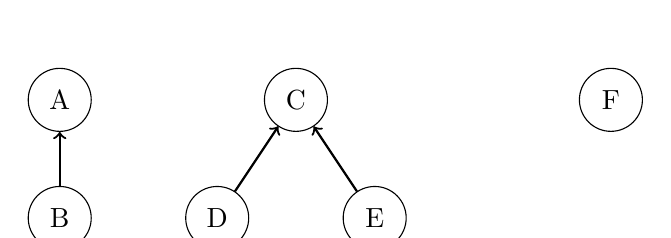
\begin{tikzpicture}[
        level distance=1.5cm,
        level 1/.style={sibling distance=2cm},
        every node/.style={circle, draw, minimum size=0.8cm}
    ]
    
    % First tree (A with child B)
    \node (A) at (0,0) {A}
        child {node (B) {B}};
    
    % Second tree (C with children D and E)
    \node (C) at (3,0) {C}
        child {node (D) {D}}
        child {node (E) {E}};
    
    % Third tree (just F)
    \node (F) at (7,0) {F};
    
    % Arrows from children to parent roots
    \draw[->, thick] (B) -- (A);
    \draw[->, thick] (D) -- (C);
    \draw[->, thick] (E) -- (C);
    
    \end{tikzpicture}
    \caption{A forest where there are three trees with representatives A, C and
    F.}
    \label{fig:forest}
\end{figure}

\begin{figure}[H]
    \centering  
    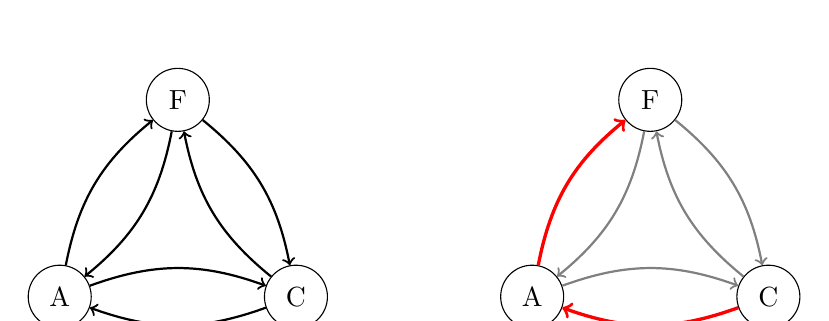
\begin{tikzpicture}[
        every node/.style={circle, draw, minimum size=0.8cm},
        every edge/.style={draw, ->, thick}
    ]
    
    % First graph
    \begin{scope}
        % Position the three nodes in a triangle
        \node (A) at (0,0) {A};
        \node (C) at (3,0) {C};
        \node (F) at (1.5,2.5) {F};
        
        % Create cycles with arrows
        \draw[->, thick] (A) to[bend left=20] (C);
        \draw[->, thick] (C) to[bend left=20] (A);
        
        \draw[->, thick] (C) to[bend left=20] (F);
        \draw[->, thick] (F) to[bend left=20] (C);
        
        \draw[->, thick] (F) to[bend left=20] (A);
        \draw[->, thick] (A) to[bend left=20] (F);
    \end{scope}
    
    % Second graph (shifted to the right with highlighted arrows)
    \begin{scope}[xshift=6cm]
        % Position the three nodes in a triangle
        \node (A2) at (0,0) {A};
        \node (C2) at (3,0) {C};
        \node (F2) at (1.5,2.5) {F};
        
        % Create cycles with arrows (normal)
        \draw[->, thick, gray] (A2) to[bend left=20] (C2);
        \draw[->, thick, red, very thick] (C2) to[bend left=20] (A2);  % Highlighted C -> A
        
        \draw[->, thick, gray] (C2) to[bend left=20] (F2);
        \draw[->, thick, gray] (F2) to[bend left=20] (C2);
        
        \draw[->, thick, gray] (F2) to[bend left=20] (A2);
        \draw[->, thick, red, very thick] (A2) to[bend left=20] (F2);  % Highlighted A -> F
    \end{scope}
    
    \end{tikzpicture}
    \caption{On the left a graph of roots from Figure \ref{fig:forest}. On the right a conflict-free set highlighted in red.}
    \label{fig:conflict-free-set}
\end{figure}

\begin{figure}[H]
    \centering  
    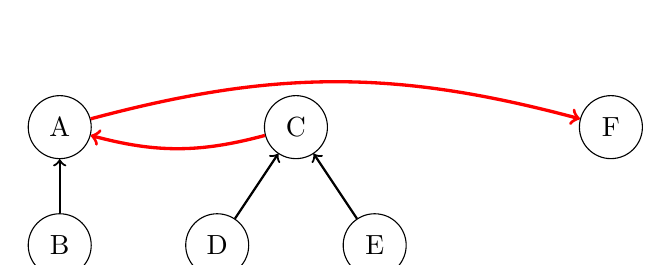
\begin{tikzpicture}[
        level distance=1.5cm,
        level 1/.style={sibling distance=2cm},
        every node/.style={circle, draw, minimum size=0.8cm}
    ]
    
    % First tree (A with child B)
    \node (A) at (0,0) {A}
        child {node (B) {B}};
    
    % Second tree (C with children D and E)
    \node (C) at (3,0) {C}
        child {node (D) {D}}
        child {node (E) {E}};
    
    % Third tree (just F)
    \node (F) at (7,0) {F};
    
    % Original arrows from children to parent roots
    \draw[->, thick] (B) -- (A);
    \draw[->, thick] (D) -- (C);
    \draw[->, thick] (E) -- (C);
    
    % New highlighted edges
    \draw[->, very thick, red] (A) to[bend left=15] (F);
    \draw[->, very thick, red] (C) to[bend left=15] (A);
    
    \end{tikzpicture}
    \caption{The forest from Figure \ref{fig:forest} after adding the
    conflict-free set from Figure \ref{fig:conflict-free-set}.}
    \label{fig:forest-after-conflict-free}
\end{figure}
\noindent The formal definition of a conflict-free set is as previous described
a set of root pairs that forms a forest.
\begin{definition}[Conflict-free Set]
  Let $F$ be a forest, $X \subseteq \{(\rho_F(v), \rho_F(u)) : (v, u) \in V
  \times V\}$ be a set of root pairs. Then $X$ is a conflict-free set in $F$
  if $(V, Y)$ is a forest.
\end{definition}
\noindent With this definition of a conflict-free set we now wish to show that
we can add all edges in a conflict-free set to a forest and still have a forest.
\begin{proposition}[Conflict-free Forest Union]\label{prop:conflict-free-forest-union}
  Let forest $F = (V, E)$ be a forest and let $X \subseteq V \times V$ be a
  conflict-free set in $F$ where $|X| = n$. Then defining the following forests:
  \begin{align*}
    F_0 &:= F \\
    F_{i} &:= (V, E_{i - 1} \cup \{(v_i, u_i)\}) \text{ for } (v_i, u_i) \in X \text{ and } 1 \leq i \leq n
  \end{align*}
  Then $F_n$ is a forest.
\end{proposition}

\begin{proof}
  Let forest $F = (V, E)$ be a forest, $X \subseteq V \times V$ be a
  conflict-free set in $F$. We will show that $F_n$ is a forest by induction
  on $i$.
  \begin{itemize}
    \item Base case: If $i = 0$ then $F_i = F_0 = F$ which is a forest.
    \item Induction hypothesis: Assume that $F_{i - 1}$ is a forest for all
    $1 \leq i < n$.  Let $(v_i, u_i) \in X$, we know that $v_i \neq v_j$ for
    all $(v_j, u_j) \in Y \backslash \{(v_i, u_i)\}$ since otherwise $(V,
    X)$ would not be a forest and $X$ would not be a conflict-free set in
    $F$. So $v_i$ will only have one parent in $F_i$ since it only appears
    once as a child in $(V, X)$. By definition all of the edges in $X$
    consists of roots in $F$, and since $(V, X)$ is a forest there are no
    cycles $y \centernot\leadsto y$ for all $y \in V$ in $F_i$. Hence $F_i$
    is a forest.
  \end{itemize}
  Thus by induction $F_n$ is a forest.
\end{proof}
\noindent We also need to show that Conflict-free Forest Union
\ref{prop:conflict-free-forest-union} satisfies Tree Union Property
\ref{def:tree-union-property}. This is done by showing that adding edges from
the conflict-free set to a forest in any order is equivalent to adding each edge
in the same order using Root Union \ref{prop:root-union}.
\begin{proposition}[Conflict-free Set Equivalence]\label{prop:conflict-free-set-equivalence}
  Let forest $F$ be a forest and let $X \subseteq V \times V$ be a
  conflict-free set in $F$ where $|X| = n$. Then defining the following forests:
  \begin{align*}
    F_0 &:= F \\
    F_{i} &:= (V, E_{i - 1} \cup \{(v_i, u_i)\}) \text{ for } (v_i, u_i) \in X \text{ and } 1 \leq i \leq n \\
    G_0 &:= F \\
    G_{j} &:= (V, E_{i - 1} \cup \{(\rho_{G_{j - 1}}(v_j), \rho_{G_{j - 1}}(u_j))\}) \text{ for } (v_j, u_j) \in X \text{ and } 1 \leq j \leq n
  \end{align*}
  Then $F_{n} \cong G_{n}$.
\end{proposition}
\begin{proof}
  Let forest $F$ be a forest, $X \subseteq V \times V$ be a conflict-free set
  in $F$. We will show that $F_n \cong G_n$. We know that for some $(v_i, u_i)
  \in X$ then $v_i \neq y$ for all  $(y, w) \in X \backslash \{(v_i, u_i)\}$
  since otherwise $(V, X)$ would not be a forest and $X$ would not be a
  conflict-free set in $F$. So all edge set unions will only give a root $v_i$
  a new parent $u_i$ once. So $\rho_{F_n}(v_i) = \rho_{F_n}(u_i)$ and
  $\rho_{G_n}(u_i) = \rho_{G_n}(v_i)$ hence $v_i$ remains in the same tree in
  both $F_n$ and $G_n$. Since this holds for all $(v_i, u_i) \in X$ it follows
  that all elements in $V$ remains in the same tree in both $F_n$ and $G_n$.
  Hence $F_n \cong G_n$.
\end{proof}
\noindent From this equivalence it will be shown that Conflict-free Forest Union
\ref{prop:conflict-free-forest-union} satisfies Tree Union Property
\ref{def:tree-union-property}.
\begin{corollary}[Conflict-free Union Satisfies Tree Union
  Property]\label{cor:conflict-free-union-satisfies-tree-union-property} Let
  forest $F$ be a forest and let $X \subseteq V \times V$ be a conflict-free set
  in $F$ where $|X| = n$. Then defining the following forests:
  \begin{align*}
    F_0 &:= F \\
    F_{i} &:= (V, E_{i - 1} \cup \{(v_i, u_i)\}) \text{ for } (v_i, u_i) \in X \text{ and } 1 \leq i \leq n
  \end{align*}
  Then for all $(v_i, u_i) \in X$ it holds that $v_i \sim_{F_n} u_i$ and $F_n$
  satisfies the properties of a tree union.
\end{corollary}
\begin{proof}
  Let forest $F$ be a forest, $X \subseteq V \times V$ be a conflict-free set
  in $F$. By proposition \ref{prop:conflict-free-set-equivalence} it holds
  that $F_n \cong G_n$ where $G_n$ is defined as in proposition
  \ref{prop:conflict-free-set-equivalence}. By proposition \ref{prop:root-union}
  it holds that for all $(v_i, u_i) \in X$ then $v_i \sim_{G_n} u_i$ and $G_n$
  satisfies the properties of a tree union. Since $F_n \cong G_n$ it follows
  that for all $(v_i, u_i) \in X$ then $v_i \sim_{F_n} u_i$ and $F_n$ satisfies
  the properties of a tree union.
\end{proof}

\noindent Now that we have established the properties of conflict-free sets we
can now define a method to find a conflict-free set from a set of root pairs.
The method chosen to find a conflict-free set is to consider an directed acyclic
graph. Such a graph fulfills one property of a forest, namely that there are no
cycles. This is ensured by ordering the edges in the graph such that for all
edges $(v, u)$ it holds that $v < u$ for some strict total order $(V, <)$. We
may do this since the equivalence classes in a forest can be represented by any
representative in the tree. Hence we can alwauys pick a total order on the
vertices in the forest.
\begin{proposition}[Ordered Edges Implies Acyclicity]\label{prop:ordered-edges-implies-acyclicity}
  Let $G = (V, E)$ be a directed graph where for all $(v, u) \in E$ it holds
  that $v < u$ for some strict total order $(V, <)$. Then $G$ has no cycles.
\end{proposition}

\begin{proof}
  Let $G = (V, E)$ be a directed graph where for all $(u, v) \in E$ it holds
  that $u < v$ for some total order $(V, <)$. Let edges $e_1, e_2, \ldots, e_m
  \in E$ where $m \geq 1$ and $e_i = (v_{i-1}, v_i)$ for $1 \leq i \leq m$ be
  some path in $G$. Since the edges are ordered it follows that:
  \begin{align*}
    v_0 < v_1 < v_2 < \cdots < v_{m - 1} < v_m
  \end{align*}
  Hence by transitivity of the total order it follows that $v_0 < v_m$. So
  $v_0 \neq v_m$ hence there are no cycles in $G$.
\end{proof}
\noindent The nice property of using a directed acyclic graph is we can now pick
out any vertices from the graph such that no two vertices have the same child.
This will ensure that the picked out edges forms a forest.

\subsection{Parallel Union-Find}
The conflict-free sets makes it is possible to define how unification in the
union-find strucutre works. If we consider that we have some forest $F = (V, E)$
and then are given a set of variables pairs $A \subseteq V \times V$ we wish to
unify these pairs such that they are equivalent in some forest $F$. We can turn
$A$ into an acyclic graph $(V, Z)$ where $Z$ only consists of root pairs from
$F$. We want to pick out a subset of $Z$ such that we unify as many of the
vertex pairs of $Z$ in $F$ as possible leading to a good time complexity of the
algorithm. All of these pairs can not be unified immediately so an algorithm
will be first derived which picks out a subset of the directed acyclic graph
$(V, Z)$ and then unifies them in $F$. To determine what a large set is we is
first need to define a notion of an edge cover that can be serve as a measure of
how many vertex pairs in $Z$ can be unified:
\begin{definition}[Edge Cover]
    Let $V$ be a set and $E \subseteq V \times V$ such that $\pi_1(E) \cup
    \pi_2(E) = V$ then $E$ is an edge cover of $V$.
\end{definition}
\noindent Using this definition we know that $V' = \pi_1(Z) \cup \pi_2(E)$ is an
edge cover of the subgraph $(V', Z)$ of $(V, Z)$. Why this is relevant is that
vertices in $V\backslash V'$ will not be unified so they are not relevant during
unification. Futhermore, the bound that will be establish is for every iteration
then atleast $\frac{|V'|}{2}$ vertices must be unified. The intuition behind
this is that every time a vertex is given a parent then it can not be given a
parent later so it has been dealt with. We can show that when we have such an
edge cover then the following inequality holds:
\begin{proposition}[Edge Cover Inequality]\label{prop:set-2-tuple-inequality}
    Let $V$ be a set and $E \subseteq V \times V$ be a edge cover of V then: 
    \begin{align*}
        |\pi_1(E)| < \frac{|V|}{2} \implies |\pi_2(E)| > \frac{|V|}{2} 
    \end{align*}
\end{proposition}
\begin{proof}
    Let $V$ be a set and $E \subseteq V \times V$ be a edge cover of V, and
    $|\pi_1(E)| < \frac{|V|}{2}$. Let $A = \pi_1(E) = \{v : (v, u) \in E\}$, $B
    = \pi_2(E) = \{u : (v, u) \in E\}$ and $C = B \backslash A$. By definition of $C$ we
    have $A \cap C = \emptyset$ so $|A| + |C| = |V|$ and since $|B| \geq |C|$ we
    can conclude that:
    \begin{align*}
        |B| \geq |C| = |V| - |A| > |V| - \frac{|V|}{2} = \frac{|V|}{2}
    \end{align*}
    Hence $|\pi_1(E)| > \frac{|V|}{2}$.
\end{proof}
\noindent This inequality tells us that if $Z$ does not resolve enough vertices,
then if we invert the edges in $Z$ then it would be possible to resolve enough
vertices. It just remains to show that inverting these edges direction will
still give an acyclic graph.  
\begin{proposition}[Inverted Acyclic Graph is Acyclic]\label{prop:inverted-acyclic-graph}
  Let $G = (V, E)$ be a directed acyclic graph. Then the inverted graph $G' =
  (V, E')$ where $E' = \{(u, v) : (v, u) \in E\}$ is also acyclic.
\end{proposition}
\begin{proof}
  Let $G = (V, E)$ be a directed acyclic graph and $G' = (V, E')$ where $E' =
  \{(u, v) : (v, u) \in E\}$ is the inverted graph. Let edges $e_1, e_2,
  \ldots, e_m \in E'$ where $m \geq 1$ and $e_i = (v_{i-1}, v_i)$ for $1 \leq
  i \leq m$ be some path in $G'$. By definition of $E'$ it follows that there
  exists edges $e'_1, e'_2, \ldots, e'_m \in E$ where $e'_i = (v_i, v_{i-1})$
  for $1 \leq i \leq m$. If there was a cycle in $G'$ then it would hold that
  $v_0 = v_m$. But since $G$ is acyclic it follows that $v_0 \neq v_m$. Hence
  there are no cycles in $G'$.  
\end{proof}
\noindent The algorithm which tries to unifies atleast $\frac{|V'|}{2}$ can now
be defined. It starts by determining if the directed acyclic subgraph $(V', Z)$
should be inverted as to give $\frac{|V'|}{2}$ vertices a parent. Afterwards 
just pick out as many pairs with a unique child.
\begin{algorithm}[Maximal Union]\label{alg:maximal-union} Let forest $F = (V,
  E)$ be a forest and let $Z \subseteq \{(\rho_F(v), \rho_F(u)) : (v, u) \in V
  \times V\}$ be a set of root pairs $F$ and $(V, Z)$ is an acyclic directed
  graph. The maximal union algorithm is defined as:
  \begin{align*}
    & \id{MaximalUnion}(F, Z) \\ 
    1. & \qquad (V, E) \leftarrow F \\
    2. & \qquad V' \leftarrow \pi_1(Z) \cup \pi_2(Z) \\
    3. & \qquad Z \leftarrow \begin{cases}
      \{(u, v) : (v, u) \in Z\} & \pi_1(Z) < \frac{|V'|}{2} \\
      Z & \pi_1(Z) \geq \frac{|V'|}{2}
    \end{cases} \\
    4. & \qquad X \leftarrow Y \subseteq Z \text{ where } |Y| = |\pi_1(Z)| \text{ and } \pi_1(Y) = \pi_1(Z) \\
    5. & \qquad G \leftarrow (V, X) \\
    6. & \qquad E \leftarrow E \cup \{(v, \rho_G(u)) : (v, u) \in X\} \\
    7. & \qquad \kw{return} \: ((V, E), Z \backslash X)
  \end{align*}
\end{algorithm}
\noindent By definition we can clealy see atleast $\frac{|V'|}{2}$ vertices are
given a parent as we wanted. It will now be shown that the added edges is a
conflict-free set so a forest is still the result.
\begin{proposition}[Maximal Union
  Correctness]\label{prop:maximal-union-correctness} Let forest $F = (V, E)$ be
  a forest and let $Z \subseteq \{(\rho_F(v), \rho_F(u)) : (v, u) \in V \times
  V\}$ be a set of root pairs $F$ and $(V, Z)$ is an acyclic directed graph.
  Then the maximal union algorithm results in a forest $F' = (V, E')$ which
  satifies the Tree Union Property \ref{def:tree-union-property} for the
  conflict-free set $X \subseteq Z$ in $F$.
\end{proposition}
\begin{proof}
  Let forest $F = (V, E)$ be a forest and let $Z \subseteq \{(\rho_F(v),
  \rho_F(u)) : (v, u) \in V \times V\}$ be a set of root pairs $F$ and $(V, Z)$
  is an acyclic directed graph. From proposition
  \ref{prop:inverted-acyclic-graph} we know that $(V, Z)$ remains an acyclic
  graph throughout the algorithm. Since $X$ is defined such that $\pi_1(X) =
  \pi_1(Z)$ and $|X| = |\pi_1(Z)|$ it follows that $X$ is a conflict-free set in
  $F$ since no vertex $v$ appears more than once as a child in $X$ i.e. $G = (V,
  X)$ is a forest. We can also conclude that $(V, \{(v, \rho_G(u)) : (v, u) \in
  X\}) \cong (V, X)$ since every child directly points to its root. So adding
  the edges in $\{(v, \rho_G(u)) : (v, u) \in X\}$ to $E$ it follows by
  corollary \ref{cor:conflict-free-union-satisfies-tree-union-property} that the
  algorithm fulfills the Tree Union Property \ref{def:tree-union-property} and
  $F' = (V, E')$ where $E' = E \cup \{(v, \rho_G(u)) : (v, u) \in X\}$.
\end{proof}
\noindent Before the time complexity of maximal union can be shown a conjecture
will be needed. A problem that occur in the analysis is the computation of
$\{(v, \rho_G(u)) : (v, u) \in X\}$. Since the forest $(V, X)$ that may be
constructed could be just a tree which is one long chain so $\rho_G(u)$ does
$O(|X|)$ work to find its parent. This problem can be solved using pointer
jumping efficiently, specifically Wyllie's List Ranking algorithm
\cite[59]{wyllie1979complexity} can be used on a forests to do $O(n \log n)$
work with $O(\log n)$ span on a forests of $n$ vertices. This is not work
efficient, you would want to do $O(n)$ work. There are list ranking algorithms
\cite{Anderson1991} which can be used on lists but it is unclear to the author
if this will work on forests but from looking at the literature it seems likely
they will work. 

\begin{conjecture}[Path Compression Time Complexity]
  Let $F = (V, E)$ be a forest then the set $\{(v, \rho_F(u)) : (v, u) \in E\}$
  can be computed in $O(|V|)$ work and $O(\log |V|)$ span.
\end{conjecture}

\noindent Now that the path compression conjecture has been established the time
complexity of maximal union can be found.
\begin{proposition}[Maximal Union Time
  Complexity]\label{prop:maximal-union-time-complexity} Let forest $F = (V, E)$
  be a forest and let $Z \subseteq \{(\rho_F(v), \rho_F(u)) : (v, u) \in V
  \times V\}$ be a set of root pairs in $F$ and $(V, Z)$ is an acyclic directed
  graph. Then the maximal union algorithm runs in $O(|Z|)$ work and $O(\log
  |Z|)$ depth.
\end{proposition}

\begin{proof}
  For step 1. it takes $O(1)$ work and $O(1)$ if we assume that $E$ is only used
  once in this function. Step 2-3. finds unique elements and can be computed
  with a parallel integer sort and a filter, assuming the encoding of vertices
  uses a fixed number of $k$-bits then this part is $O(|Z|)$ work and $O(\log
  |Z|)$ span. Step 4. can be implemented by a parallel integer sort on the first
  element of each pair in $Z$ followed by a parallel filter that selects the
  first occurrence of each unique first element, this takes $O(|Z|)$ work and
  $O(\log |Z|)$ depth. Step 6. takes $O(|X|)$ work and $O(\log |X|)$ depth to do
  path compression and add these edges to $E$. Step 7. takes $O(|Z|)$ work and
  $O(\log |Z|)$ depth to compute the set difference $Z \backslash X$ by a
  filter. Hence the total work is $O(|Z|)$ and the total depth is $O(\log |Z|)$.
  Hence the left maximal conflict-free set algorithm runs in $O(|Z|)$ work and
  $O(\log |Z|)$ depth.
\end{proof}
\noindent Now the time complexity is known we can finally give the algorithm for
parallel union which performs bulk unification making a set of $A$ pair vertices
become equivalent in the final forest. The way the algorithm works is by
constructing a directed acyclic graph of roots from $A$ which will be called
$Z$. Then have a loop with the invariant that $(V, Z)$ is an directed
acyclic graph. Then in the loop body simply perform maximal union and turn the
remaining uninserted edge of $Z$ into an directed acyclic graph. Continue till
$Z$ is empty and then $F$ is the final forest where all pairs of $A$ has been
unified.

\begin{algorithm}[Parallel Tree Union]\label{alg:parallel-tree-union}
  Let forest $F = (V, E)$ be a tree and let $A \subseteq V \times V$ be a set of pairs
  of elements in $V$ that will be unioned in parallel. The parallel tree union
  algorithm is defined as:
  \begin{align*}
    & \id{ParallelTreeUnion}(F, A) \\
    1. & \qquad Z_p \leftarrow \{(\rho_F(v), \rho_F(u)) : (v, u) \in A \land \rho_F(v) \neq \rho_F(u)\} \\
    2. & \qquad Z \leftarrow \{(\min \{v, u\}, \max \{v, u\}) : (v, u) \in Z_p\} \\
    3. & \qquad \kw{while }~|Z| > 0~\kw{do} \\
    4. & \quad \qquad (F, Z_q) \leftarrow \id{MaximalUnion}(F, Z) \\
    5. & \qquad \quad Z_r \leftarrow \{(\rho_{F}(v), \rho_{F}(u)) : (v, u) \in Z_q \land \rho_{F}(v) \neq \rho_{F}(u)\} \\
    6. & \qquad \quad Z \leftarrow \{(\min \{v, u\}, \max \{v, u\}) : (v, u) \in Z_r\} \\
    7. & \qquad \kw{return} \: F
  \end{align*}
\end{algorithm}
\noindent First of all we have to establish that the actual algorithm produces
the correct output, as in it fullfills the Tree Union property \ref{def:tree-union-property}.

\begin{proposition}[Parallel Tree Union Correctness]
  Let forest $F = (V, E)$ be a tree and let $A \subseteq V \times V$ be a set of
  pairs of elements in $V$ that will be unioned in parallel. Then the parallel
  tree union algorithm returns a forest $F' = (V, E')$ where for all $(v, u) \in
  A$ it holds that $v \sim_{F'} u$.
\end{proposition}
\begin{proof}
  Step. 1-2 creates a directed acyclic graph and it will be shown that this
  suffices 
  
  The loop in Step. 3-6 has the following invariants where we enumerate $i$th 
  \begin{enumerate}
    \item $Z_i$ is an directed acyclic graph.
    \item $|Z_i| \geq |Z_{i + 1}|$.
  \end{enumerate}
   .
\end{proof}

\begin{proposition}[Parallel Tree Union Time Complexity]
  Let forest $F = (V, E)$ be a tree and let $A \subseteq V \times V$ be a set
  of pairs of elements in $V$ that will be unioned in parallel. Then the
  parallel tree union algorithm runs in $O(|A|^2)$ work and $O(|V|)$ span.
\end{proposition}

\subsection{Union by Size and Rank}

\subsection{Parallel Union-Find Imrovements}

\section{Implementation}

\subsection{Interface}
The interface of the union-find structure consists of a data-type which is the
union-find structure itself. The elements in the union-find structure are
represented as integers. These integers are called \textit{handles} and are used
to refer to the elements in the union-find structure. The union-find structure
is initialized with a fixed number of elements $n$ where the handles are in the
range $[0, n - 1]$ so they can be used as indices in an array of size $n$. When
exposing these elements to a user then they are abstract datatypes such that the
the user cannot do uninteneded operations on the handles or give invalid handles
to the union-find structures operations.

The operations supported are \id{find} and \id{union}. The find operation takes
a handle and returns the representative which is also a handle. This can be used
to check if two elements are in the same set or is ``equivalent'' by checking if
their representatives are the same. The union operation takes two handles such
that they have the same representative and are therefore in the same set or to
be considered ``equivalent''. These operations are done in bulk meaning that the
find operation takes an array of handles and union can union multiple pairs of
handles in parallel.

\subsection{Union-find}
The first and simplest implementation of the union-find structure is based on
the basic parallel tree union algorithm \ref{alg:parallel-tree-union}. It will
be extremely inefficient if we do not apply normalization of a left maximal
union since you may produce long chains of elements pointing to each other which
will make the find operation very expensive. This can be solves by compressing
the paths during the find operation such that all elements point directly to
their representative after a left maximal union. This will not optimize a
sequence of union or find operations but assuming you only have to do one
singular bulk union followed by multiple bulk find operations it will be
efficient.

\subsubsection{Data type}
A simple union-find structure can be implemented using an array indices which
where the index represents the element/handle and the value at that index is
the parent of that element. If the value at that index is a special value which
is the highest possible integer value then that element is a root and therefore
its own representative. In pseudo code we denote this as an array of integers:
\begin{flalign*}
  & \id{parents} : [n]\Int &
\end{flalign*}
Initially all of these values are set to \id{none} which indicates that all
elements are their own representative. Here \id{none} is defined as an integer
$n \geq \id{none}$.

\subsubsection{Find}
To implement the find operation we can simple do a parallel map over all
elements to find their representative by a simple loop that follows the
parent pointers until a root is found. Since this operation does not modify the
structure we can simplify implement it as so:
\begin{flalign*}
  & \kw{def}~\id{find\_one}~(\id{parents} : [n]\Int)~(\id{handle} : \Int) = & \\
  & \qquad \If~\id{parents}[\id{handle}] = \id{none} & \\
  & \qquad \kw{then}~\id{handle} & \\
  & \qquad \Else~\id{find}~\id{parents}~(\id{parents}[\id{handle}]) &
\end{flalign*}
Then the bulk find operation can be implemented as:
\begin{flalign*}
  & \kw{def}~\id{find}~(\id{parents} : [n]\Int)~(\id{handles} : [m]\Int) = & \\
  & \qquad \kw{map}~(\id{find\_one}~\id{parents})~\id{handles} &
\end{flalign*}

\subsubsection{Union}
The union operation can be implemented using the parallel tree union algorithm
\ref{alg:parallel-tree-union} but due to its abstract nature one must figure out
how to make it work in the concrete implementation.

The initial step is to find the representatives of all handle pairs that will
be unioned. This can be done by a map followed by a filter to remove pairs
where both elements already have the same representative:
\begin{flalign*}
& \kw{def}~\id{find\_pairs}~(\id{parents} : [n]\Int)~(\id{pairs}: [m](\Int, \Int)) = & \\
& \qquad \Let~\id{find\_one\_pair}~(v, u) = & \\
& \qquad \quad (\id{find\_one}~parents~v,~\id{find\_one}~parents~u) & \\
& \qquad \In ~(\kw{filter}~(\lambda (v, u) \to v \neq u) \circ \kw{map}~\id{find\_one\_pair})~pairs &
\end{flalign*}
The next step is we want to order all pairs such that it forms an acyclic directed graph. This can be done by simply ordering each pair such that the
first element is always less than the second element:
\begin{flalign*}
& \kw{def}~\id{order}~(\id{pairs} : [m](\Int, \Int)) = & \\
& \qquad \kw{map}~(\lambda (v, u) \to \If~v < u~\kw{then}~(v, u)~\Else~(u, v))~\id{pairs} &
\end{flalign*}
Now left maximal union can be performed on the ordered pairs, we do this simply
by selecting one parent for each unique first element in the pairs. This can be
done by a reduce by index operation using \id{min} as the reduction operator.
Now we just have to partition the pairs into those that were successfully
unioned and those that were not. The ones that were not unioned are those where
the parent did not change.

There is just one problem with this approach and it is that this may construct
one long chain of elements pointing to each other which will make future find
operations expensive. This can be solved by normalizing the structure after the
left maximal union such that all elements that were given a new parent now point
directly to their representative. This results in the following left maximal
union implementation:
\begin{flalign*}
& \kw{def}~\id{left\_maximal\_union}~(\id{parents} : [n]\Int)~(\id{pairs} : [m](\Int, \Int)) = & \\
& \qquad \Let~(l, r) = \id{unzip}~\id{pairs} & \\
& \qquad \Let~\id{parents'} = \id{reduce\_by\_index}~\id{parents}~\id{min}~\id{none}~l~r & \\
& \qquad \Let~(\id{remaining}, \id{done}) = \id{partition}~(\lambda (i, p) \to \id{parents'}[i] \neq p)~\id{pairs} & \\
& \qquad \Let~\id{parents''} = \id{normalize}~\id{parents'}~(\kw{map}~(\lambda (x, y) \to x)~\id{done}) & \\
& \qquad \In ~(\id{parents''}, \id{remaining}) &
\end{flalign*}
The normalization step can be implemented by using the wyllie list ranking
algorithm \cite[59]{wyllie1979complexity} to compress the paths in the
union-find structure. The modification is instead of checking if the parent does
not exists we have to check if it is a root or the grandparent is a root then we
are done.
\begin{flalign*}
& \kw{def}~\id{normalize\_step}~(\id{is} : [m]\Int)~(\id{parents} : [n]\Int) = & \\
& \qquad \Let~\id{next}~(\id{handle} : \Int) = & \\
& \qquad \quad \If~\id{parents}[\id{handle}] = \id{none} & \\
& \qquad \quad \kw{then}~\id{handle} & \\
& \qquad \quad \Else~\If~\id{parents}[\id{parents}[\id{handle}]] = \id{none} & \\
& \qquad \quad \kw{then}~\id{parents}[\id{handle}] & \\
& \qquad \quad \Else~\id{parents}[\id{parents}[\id{handle}]] & \\
& \qquad \In~\id{scatter}~\id{parents}~\id{is}~(\kw{map}~\id{next}~\id{is}) &
\end{flalign*}
Then we just have to repeat this process $\lceil \log_2 m \rceil$ times to
ensure that all paths are compressed:
\begin{flalign*}
& \kw{def}~\id{normalize}~(\id{parents} : [n]\Int)~(\id{is} : [m]\Int) = & \\
& \qquad \Let~\id{loop}~(\id{parents'} : [n]\Int)~(\id{is'} : [m]\Int)~(\id{count} : \Int) = & \\
& \qquad \quad \If~\id{count} = 0 & \\
& \qquad \quad \kw{then}~\id{parents'} & \\
& \qquad \quad \Else~\id{normalize\_step}~\id{is'}~\id{parents'} & \\
& \qquad \quad \In ~\id{loop}~\id{parents'}~\id{ps'}~(\id{count} - 1) & \\
& \qquad \In ~\id{loop}~\id{parents}~\id{is}~\lceil\log_2 m\rceil &
\end{flalign*}
The last step in the parallel tree union algorithm is to swap the pairs such
that we can perform left maximal union again on the inverted pairs. This takes
the acyclic directed graph formed by the remaining pairs and inverts all edges:
\begin{flalign*}
  & \kw{def}~\id{swap} ~(\id{pairs} : [n](\Int, \Int)) = & \\
  & \qquad \Map ~(\lambda (v, u) \to (u, v))~\id{pairs} &
\end{flalign*} 
Now we have all the functions needed to implement the union operation:
\begin{flalign*}
& \kw{def}~\id{union}~(\id{parents} : [n]\Int)~(\id{pairs} : [m](\Int, \Int)): [n]\Int = & \\
& \qquad \text{let } pairs =
\end{flalign*}


\subsection{Union by Rank}

\subsection{Union by Size}


\section{Tests}


\section{Benchmarks}


\section{Examples}

\subsection{Region Labeling}

\subsection{Type Constraint}

\section{Conclusion}

\end{document}
